\chapter{General Analysis Strategy}
\label{chap:AnaStrategy}
\section{ R-Parity Conserving SUSY Searches in Regions with Large Mass Splittings }

\indent In R-parity conserving SUSY searches, the sought-after super-symmetric particles are produced in pairs.  Each particle decays via a chain that ends in a stable, lightest super-symmetric particle (LSP).  If the LSP is weakly interacting, it can not be directly detectable by the ATLAS detector and must be inferred from transverse momentum conservation as \MET.  The rest of the products from the decay chain will be a series of SM particles.  ~\\

\indent All searches must distinguish between signal SUSY processes and background SM processes that mimic the signal detector signature.  Most search methods often place a special emphasis on identifying the LSP as this is the one decay product that is unique to SUSY events.  Practically this generally means searching for events with large amount of \MET.  \\

\indent In regions with a large mass splitting between sparticle and LSP, the decay of the original sparticle generates large amounts of momentum for the LSP.  Searches targeting high sparticle masses with large mass splittings therefore target the large amount of $\MET$ generated by the LSP, as a method to separate signal from background. The $\met$ distribution for stop signals with $(m_{\stop}, m_{\ninoone}) = (1000 \gev,1 \gev)$ and $(600 \gev, 300 \gev)$ is shown in figure \ref{fig:presel:MET1}. ~\\

\begin{figure}[h!]
%\begin{center}
\centering
    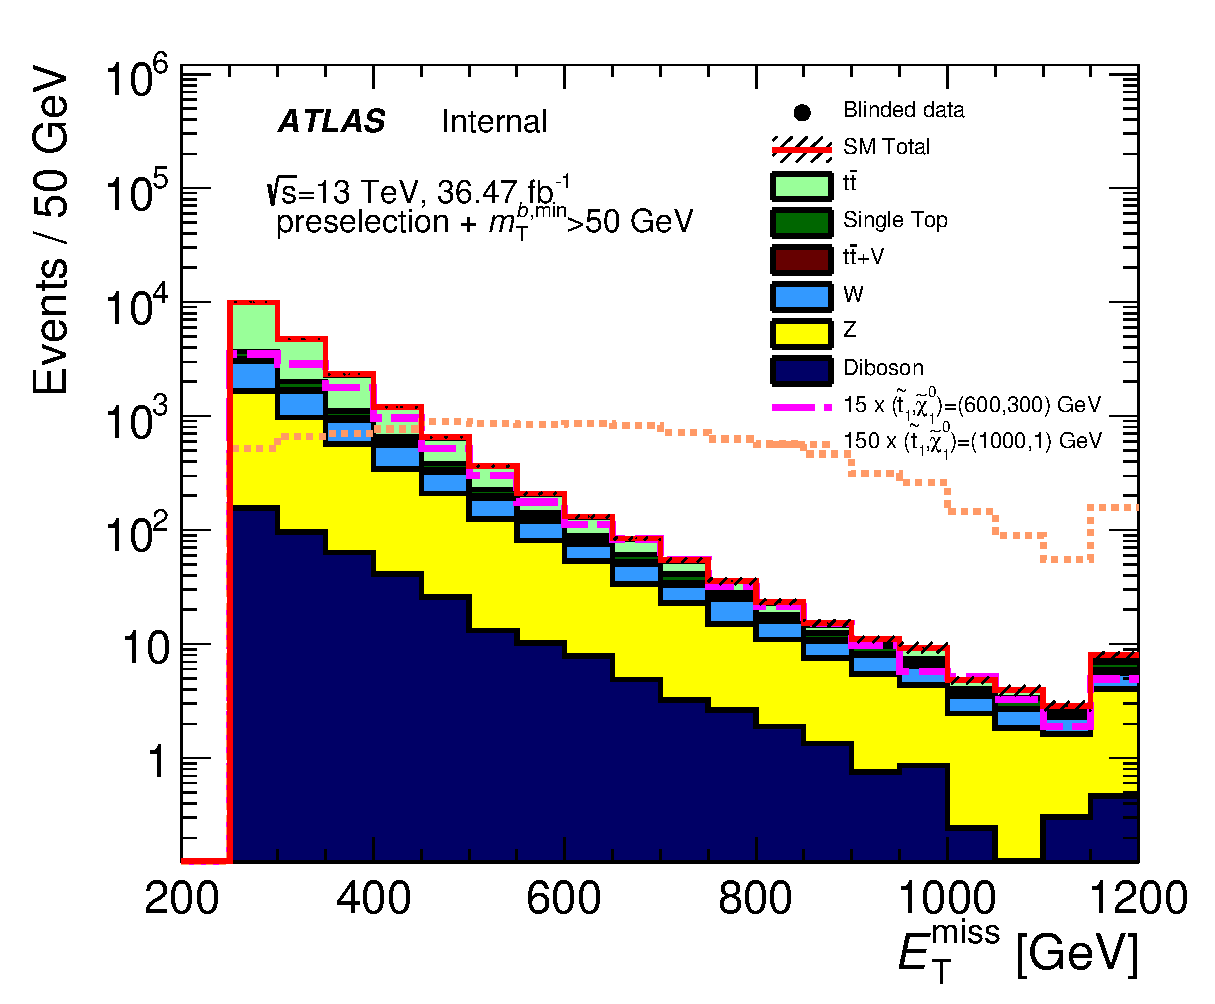
\includegraphics[width=0.85\textwidth]{figures/preselection/Met_preCutSRPlot_withRatio_log.eps}\hspace{0.05\textwidth}
\caption{ $\met$ distribution for $(m_{\stop}, m_{\ninoone}) = (1000 \gev,1 \gev)$ and $(600 \gev, 300 \gev)$ stop signal and expected SM background.  The signal cross section has been scaled up by 150 and 15 respectively for better visibility.  Basic selections ensuring well reconstructed $\met$, no leptons, and minimal jet multiplicity requirements are applied.  Details on selections can be found in \cite{stop0LCONF} }
\label{fig:presel:MET1}
%\end{center}
\end{figure}

\indent Searches often use other kinematic variables that also depend on $\met$.  Some examples include the $\mtbmax$ and $m_{eff}$ defined in equations \ref{eqn:mtbmax} and \ref{eqn:meff}. \\

\begin{equation}
%\begin{align}
\mtbmax = \sqrt{  (E_{T,b} +\met )^2 - ( \vec{p}_T,b + \vec{E}_{T}^{miss} )^2 }
\label{eqn:mtbmax}
%\end{align}
\end{equation}

\begin{equation}
%\begin{align}
m_{eff} =  \met + \sum_{visible~objects} \pt 
\label{eqn:meff}
%\end{align}
\end{equation}

\indent $\mtbmax$ is the transverse mass between $\met$ and the b-jet that is furthest away in $\phi$ from $\met$.  $m_{eff}$ is the scalar sum of all visible object $\pt$ and $\met$.  While both variables capture additional kinematic information, both are very correlated with the total magnitude of $\met$.  The $\mtbmax$ distribution for $(m_{\stop}, m_{\ninoone}) = (1000 \gev,1 \gev)$ and $(600 \gev, 300 \gev)$ stop samples is shown in figure \ref{fig:stopMtbmin}.  The $m_{eff}$ distribution for gluinos is shown in figure \ref{fig:gluino_meff}.  SM backgrounds correspond to the solid stacked histograms. \\

\begin{figure}[htb]
  \begin{center}
    \begin{subfigure}[a]{0.33\textwidth}
        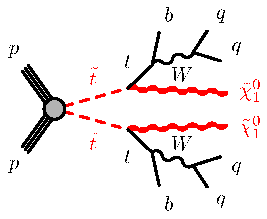
\includegraphics[width=\textwidth]{figures/feynDiag/stst-bqqbqqN1N1-tt.eps}%\hspace{0.05\textwidth}
                \caption{ }
    \end{subfigure}
    \begin{subfigure}[a]{0.45\textwidth}
        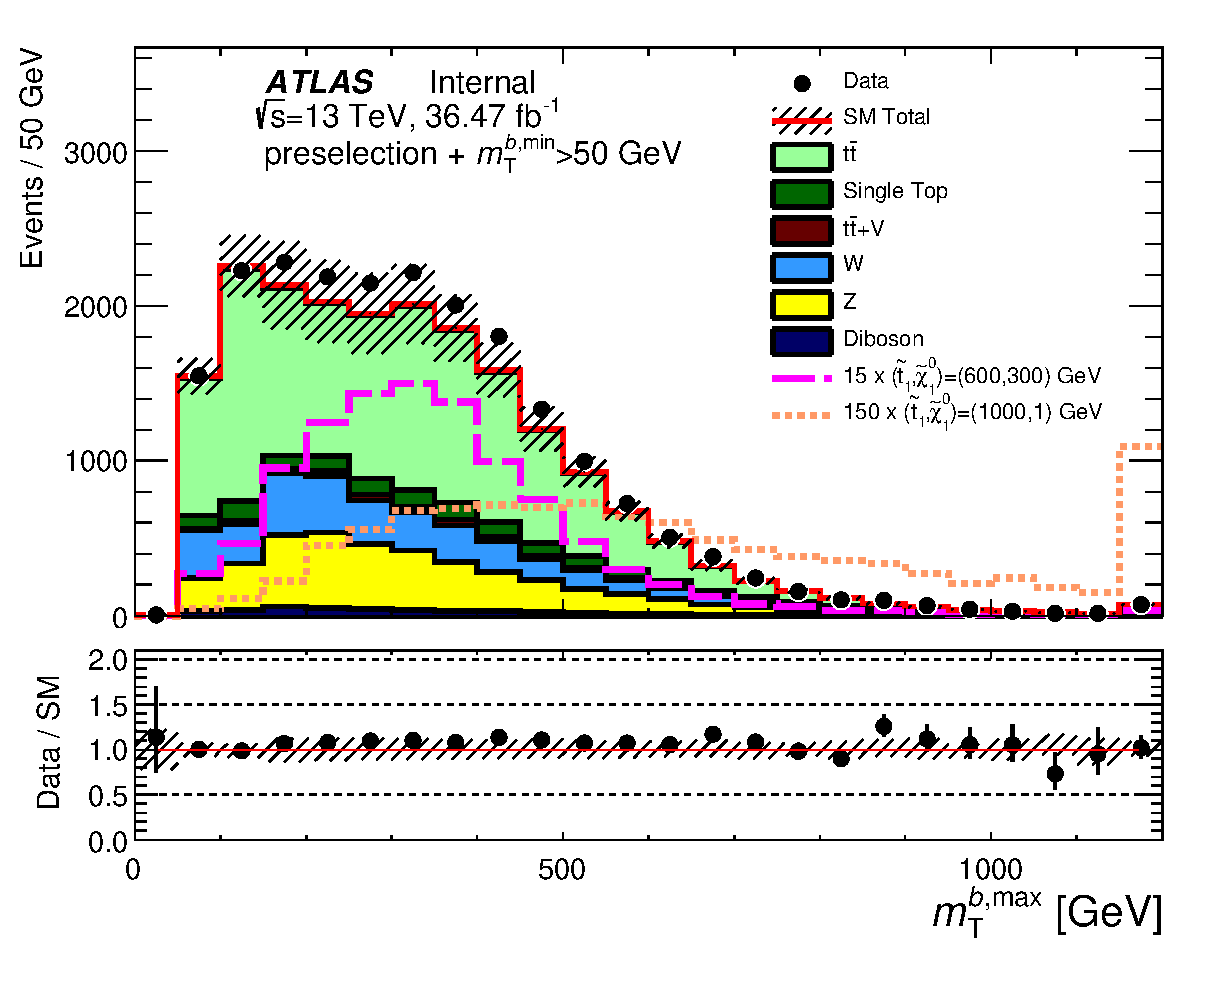
\includegraphics[width=\textwidth]{figures/preselection/MtBMax_preCutSRPlot_withRatio.eps}
                \caption{ }
    \end{subfigure}
\caption{ (a) Feynman diagram for stop production and decay. (b) \mtbmax distribution for $(m_{\stop}, m_{\ninoone}) = (1000 \gev,1 \gev)$ and $(600 \gev, 300 \gev)$ samples after lose selections for $\met>250 \gev$, zero leptons and at least four jets.  \cite{stop0LCONF} }
\end{center}
\label{fig:stopMtbmin} 
\end{figure}

\begin{figure}[htb]
  \begin{center}
    \begin{subfigure}[a]{0.33\textwidth}
        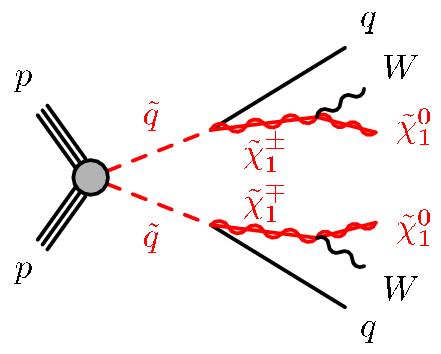
\includegraphics[width=\textwidth]{figures/feynDiag/gluino_onestep.png}%\hspace{0.05\textwidth}
                \caption{ }
    \end{subfigure}
    \begin{subfigure}[b]{0.45\textwidth}
        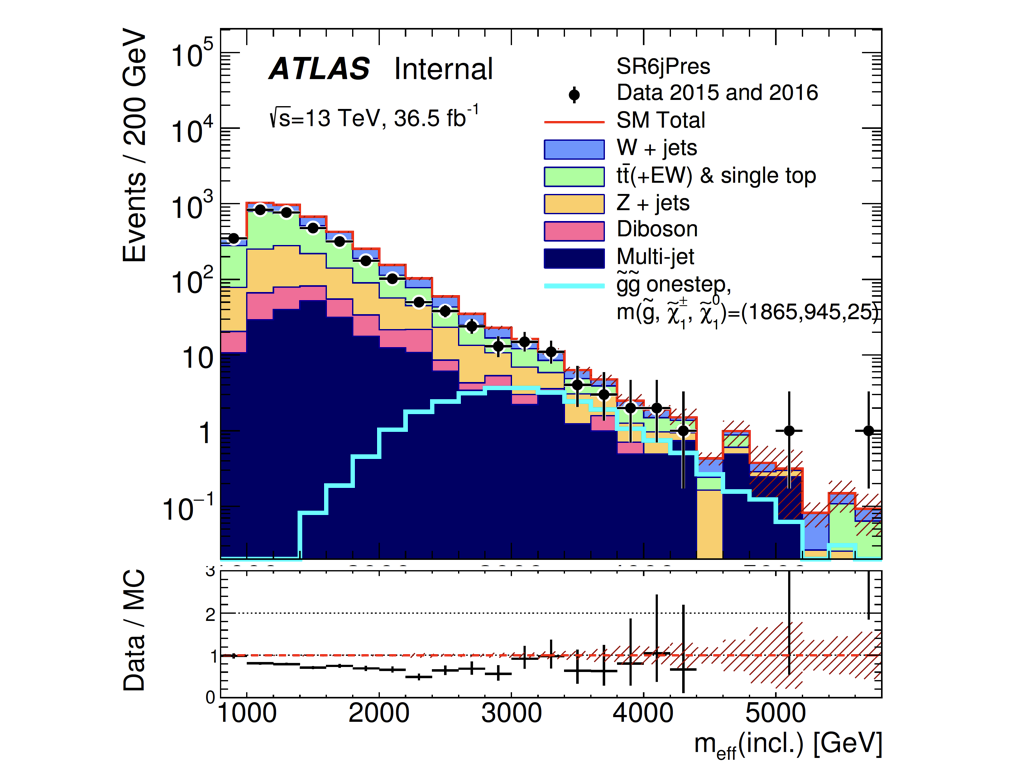
\includegraphics[width=\textwidth]{figures/strategy/gluino_meff.png}
                \caption{ }
    \end{subfigure}
\caption{ (a) Feynman diagram for gluino production and decay. (b) $m_{eff}$ distribution for gluino $(m_{\gluino}, m_{\chinopm}, m_{\ninoone}) = (1865 \gev, 945 \gev, 25 \gev)$ after lose selections for $\met>250 \gev$, zero leptons and at least six jets.\cite{SUSYinclusive0L} }
\end{center}
\label{fig:gluino_meff} 
\end{figure}

\indent Both distributions have large separation power between signal and SM backgrounds.  By making kinematic selections on these sensitive variables, ATLAS and CMS searches are able to gain sensitivity to high sparticle masses with small production cross sections.  For example, current ATLAS and CMS searches can exclude stops to upwards of 1 $\tev$. \\


\section{R-Parity Conserving SUSY Searches in Compressed Regions}


\indent When the mass splitting between the original sparticle and its decay products becomes small, the sparticle has little energy to generate momenta in its decay products.  The result is LSPs with low momenta.  The traditional strategy of searching for events with large amount of $\MET$ therefore fails in this region of parameter space.  This problem is ubiquitous to all regions with small mass splittings.  We refer to all such regions as compressed regions.  ~\\

\indent  In our analysis, the super-partner of the top, the stop is expected to decay into a neutralino and top.  When the stop mass is close to that of the top mass plus the neutralino mass, both the top and neutralino gain very little momenta from the decay.  The invisible neutralinos in turn generate very little missing transverse energy.  This leaves only the visible tops, which are mimicked by SM ttbar. \\

\indent Traditional search methods depend on variables that are highly correlated with the total magnitude of $\met$ such as $\mtbmax$ and $m_{eff}$.  Therefore traditional methods fail to separate stops from SM ttbar, which has 50 to 300 times the production cross-section of stops in the region of interest.  \\ %A High-Luminosity LHC study projects a 2$\sigma$ exclusion limit up to a stop mass of 500 $\gev$ with 300 $\ifb$ of data in this region.\cite{HLLHC_stop} The projected p-value as a function of stop mass for 300 and 3000 $\ifb$ of data is given in figure \ref{fig:HL_LHC:p_value} \\

%\begin{figure}[h!]
%  \centering
%	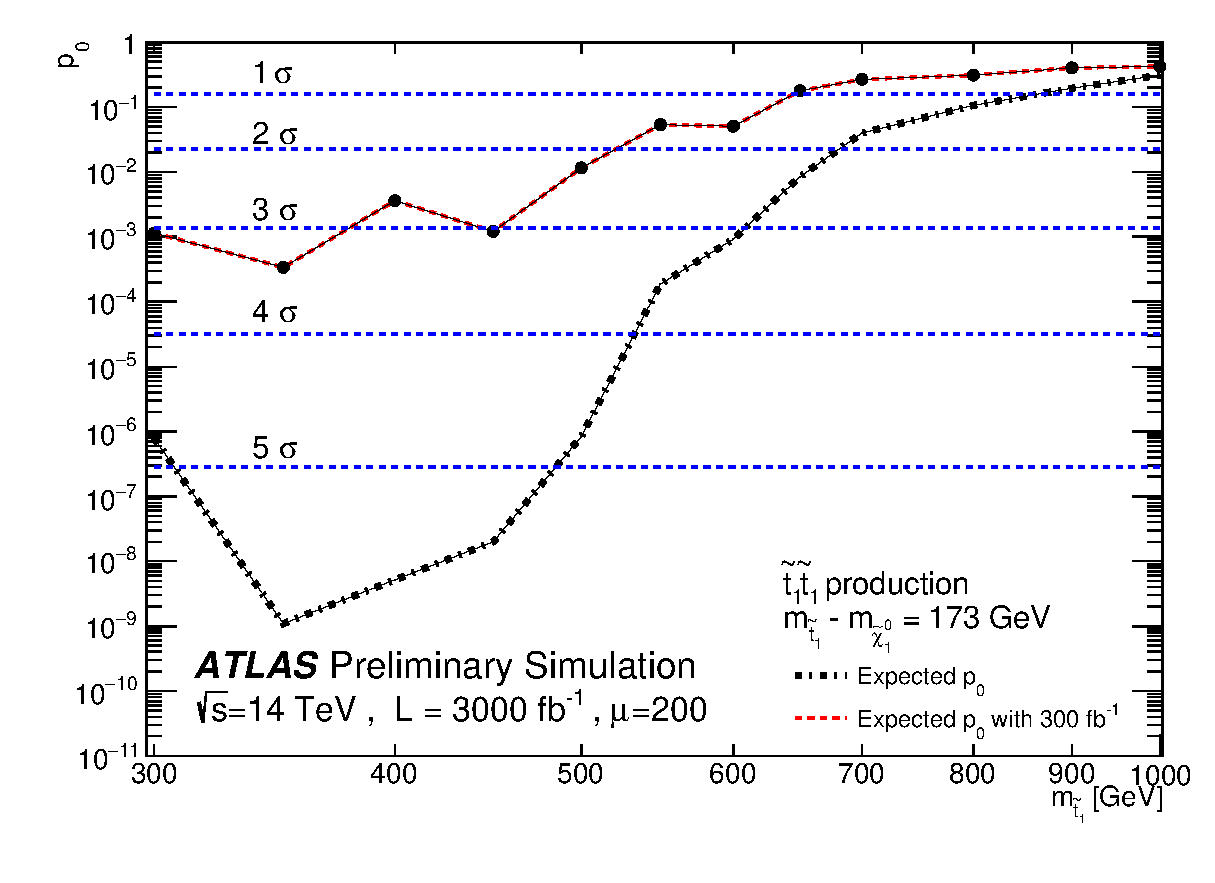
\includegraphics[width=0.65\textwidth]{./figures/strategy/HLLHC_pvalue.eps}
%\caption{Projected HL-LHC sensitivity to the $\Delta m = m_t$ region with 300 and 3000 $\ifb$ of data.  Sensitivity is quantified in terms of the p-value $p_0$.  2 sigma exclusion is reached for stop masses below 500 $\gev$ with 300 $\ifb$. Figure taken from \cite{HLLHC_stop }}
%\label{fig:HL_LHC:p_value}
%\end{figure}

\indent However, the soft decay products can gain additional momenta if the entire system is boosted by strong initial state radiation (ISR).  The goal of the traditional searches has always been to identify the presence of the LSPs and use their presence to distinguish between signal and background.  Instead of targeting events with large amount of $\MET$, we use the correlations between the LSP momenta and any ISR jets to identify LSPs in compressed regions.\cite{Pheno1,Pheno2}  Because LSPs gain little momenta from stop decays, the correlation between ISR and LSPs in compressed regions tend to be extremely strong.  By targeting the correlations between ISR and $\met$ instead of the total magnitude of $\met$, we effectively turn a weakness of the compressed region into a strength. \\

\indent For the $p p \rightarrow \antibar{\stop} \rightarrow t\ninoone\tbar\ninoone$ process, the relationship is given by equation \ref{eqn:theory_MET_ISR}. This ratio between the invisible decay products and the total ISR $\pt$ is called \RISR. \\

%\begin{equation}
\begin{align}
\MET \equiv p_{\ninoone\ninoone,~T}^{~\mathrm{lab}} \sim \gamma_{\stop\stop}^{~\mathrm{lab}} \beta_{\stop\stop}^{~\mathrm{lab}} E_{\ninoone\ninoone}^{~\stop\stop} 
\sim \frac{\PTISR}{m_{\stop\stop}} 2\gamma_{\stop}^{\stop\stop} m_{\tilde{\chi}} \sim
\PTISR \frac{ 2\gamma_{\stop}^{\stop\stop} m_{\tilde{\chi}} }{ 2\gamma_{\stop}^{\stop\stop} m_{\stop} } \sim
\PTISR \frac{m_{\ninoone}}{m_{\stop}}\implies\\
\RISR \equiv \frac{\MET}{\PTISR} \sim \frac{m_{\ninoone}}{m_{\stop}}~,\quad\quad\quad\quad\quad\quad\quad\quad\quad\quad\quad\quad
\label{eqn:theory_MET_ISR}
\end{align}
%\end{equation}

\indent The ratio between $\MET$ and ISR $\pt$ is proportional to the ratio between the mass of a single LSP and original sparticle.  Its interesting to note that the back-to-back boost between the two original stops does not affect the correlation between the observable \MET and ISR $\pt$.  Although the LSP's can individually gain momenta from the sparticles boosting against one another, the back-to-back momenta will exactly cancel resulting in zero measurable $\MET$.  \\

\indent The di-LSP system only gains $\pt$ by inheriting it from the boost by the ISR system on the two sparticles.  The fraction of the momenta that is inherited by the di-LSP system is exactly $\frac{m_{LSP}}{m_{sparticle}}$ if the sparticle decay gives no additional momentum to the LSP.  \\

\indent Figure \ref{ig:stop_400_227_ISR_MET_truth} shows the correlation between the $\RISR$ ratio in $p p \rightarrow \antibar{\stop} \rightarrow t\ninoone\tbar\ninoone$ simulation for two different stop masses (350 and 550 $\gev$) as predicted by equation \ref{eqn:theory_MET_ISR}.  The $\Delta m$ between stop and neutralino is $173 \gev$ or 550 $\mev$ from the top mass in both cases.  Both stop samples sharply peak at exactly $m_{\ninoone}/m_{\stop}$ with a gaussian width of approximately 4 percent.  No detector resolution effects were included in the simulation and only the all hadronic decay channel was considered. \\

\begin{figure}[h!]
  \centering
	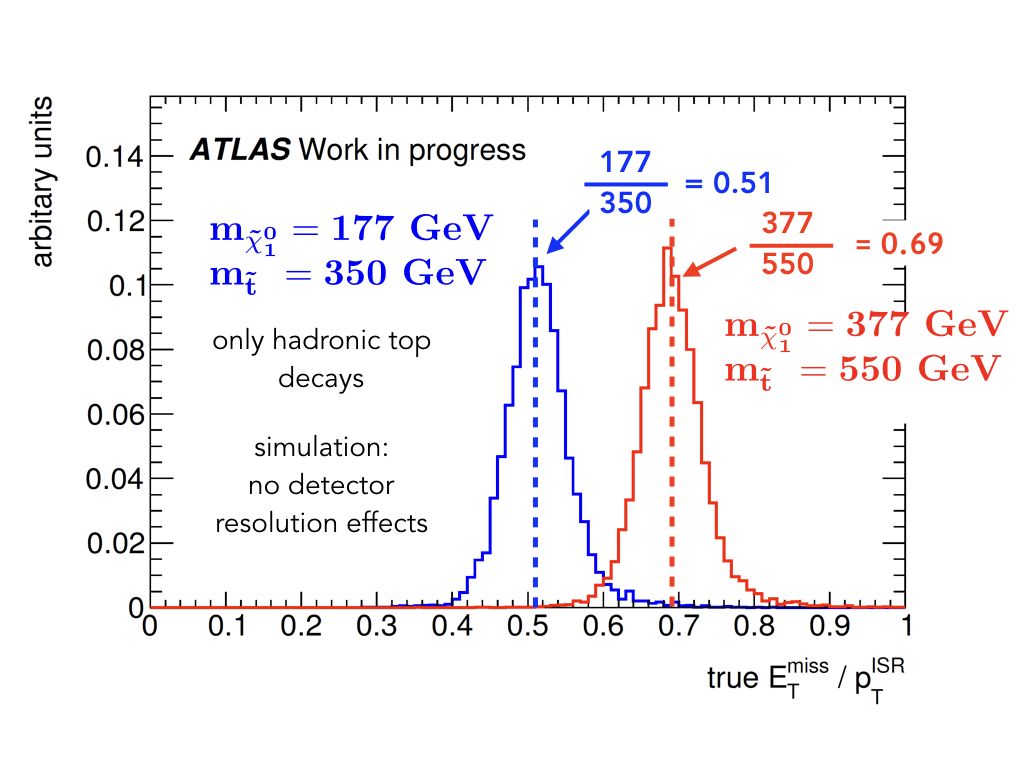
\includegraphics[width=0.65\textwidth]{./figures/strategy/RISR_truth.png}
\caption{Correlation between the $\RISR$ ratio in simulation for two different stop masses.  Both stop samples peak sharply at $m_{\ninoone}/m_{\stop}$ with only a gaussian width of 4 percent.  Deviation from the preferred ratio is limited by the top width, as the top must be pulled off shell to generate phase space. No detector resolution effects where included and only the all hadronic decay channel was considered.}
\label{fig:stop_400_227_ISR_MET_truth}
\end{figure}

\indent The ISR and $\met$ correlations also exist in direction.  ISR and $\met$ are necessarily back-to-back, because the neutralinos recoil in the opposite direction as the ISR.  \\%In comparison, the neutrino gains significant momentum directly from the top decay in ttbar background and their correlation with ISR is not as absolute.  \\

\indent The relationship between the decay products and ISR also has an additional benefit of being model independent.  This correlation is dictated solely by relativistic kinematics rather than the underlying QFT of any particular model.  The decay products' momentum and direction are determined mostly by two things, how heavy the decay products are and how hard they are kicked by the ISR.  \\

\indent We identify ISR by finding the axis of maximum back-to-back $\pt$ in the event.  The thrust axis should mimic the axis of back-to-back boost between the ISR and sparticle systems in events with strong ISR because the ISR and sparticle boost represents the single largest back-to-back kick in events with strong ISR.  \\

\indent A schematic representation of the roles of the thrust axis in stop plus strong ISR events can be seen in figure \ref{fig:ISR:ttbar_sig_example}. \\

\begin{figure}[h!]
  \centering
	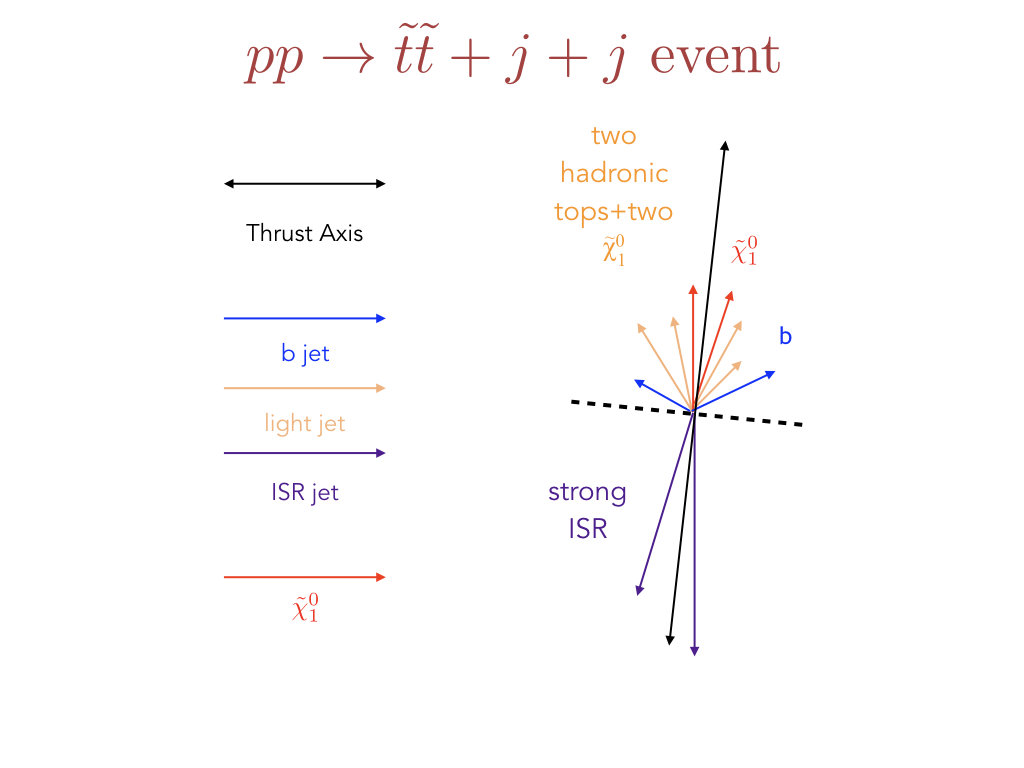
\includegraphics[width=0.85\textwidth]{./figures/strategy/ISR_signal.png}
	\caption{Schematic depictions of stop plus strong ISR event kinematics.  The thrust axis approximates the direction of back-to-back boost between ISR and stop decay products.  The hemisphere containing $\met$ also contains most of the other stop decay products.  The hemisphere opposite the $\met$ contains the energetic ISR jets. }
	\label{fig:ISR:ttbar_sig_example}
\end{figure}

\indent We divide the event into two hemispheres according to the thrust axis.  The hemisphere with $\met$, called the sparticle hemisphere, is expected to contain most stop decay products. The hemisphere opposite the $\met$ should contain the energetic ISR jets.  The accurate ISR identification algorithm preserves the sharp correlations between ISR and $\met$.  \\

\indent Other kinematic properties of the two hemispheres can also be used to separate signal from background.  For example the number of jets in the sparticle system $\NjV$ and the total transverse mass $\MS$ of the sparticle hemisphere are both expected to be larger in signal.  The $\NjV$ and $\MS$ distributions for signal and SM backgrounds are shown in figure \ref{fig:presel:NjV} \ref{fig:presel:MS}. \\

\begin{figure}[htb]
  \begin{center}
    \begin{subfigure}[a]{0.45\textwidth}
        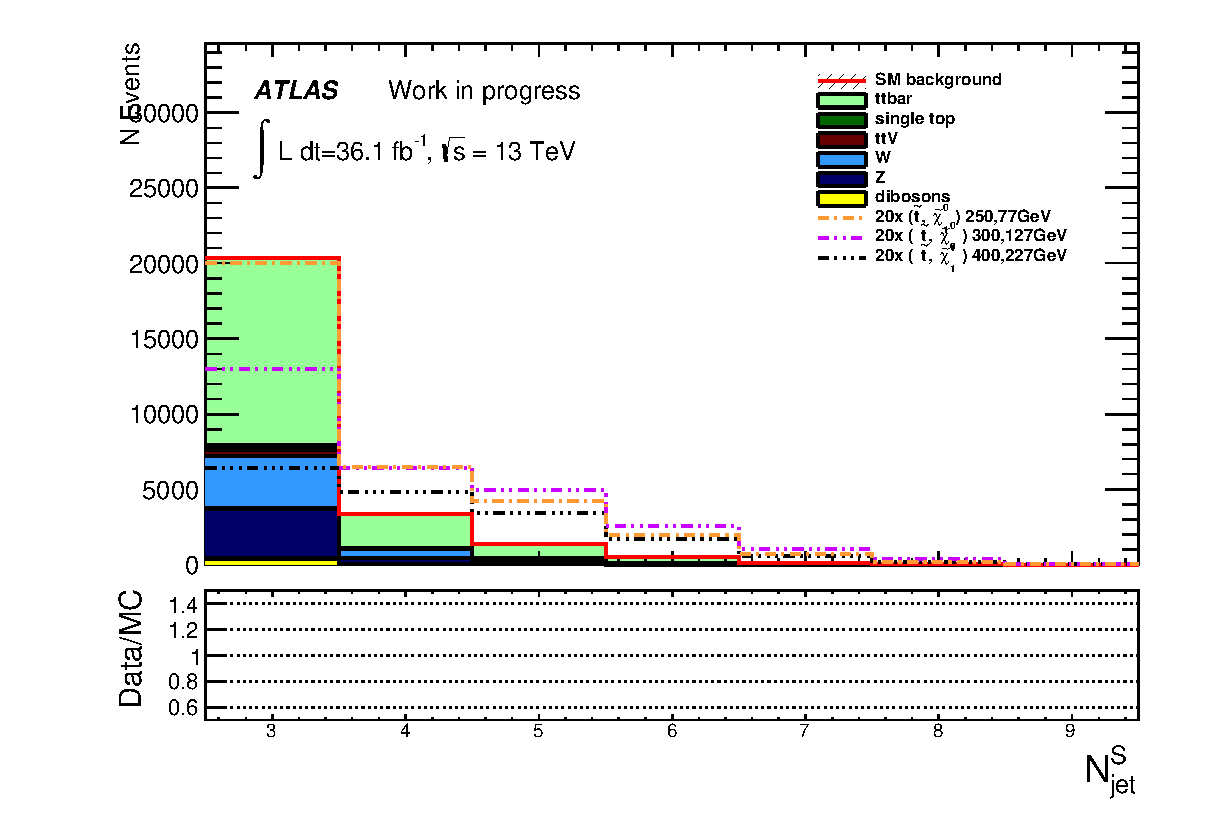
\includegraphics[width=\textwidth]{figures/plotSR/SR_ND1_NjV_0SR.eps}%\hspace{0.05\textwidth}
        \caption{ }
    \end{subfigure}
    \begin{subfigure}[b]{0.45\textwidth}
        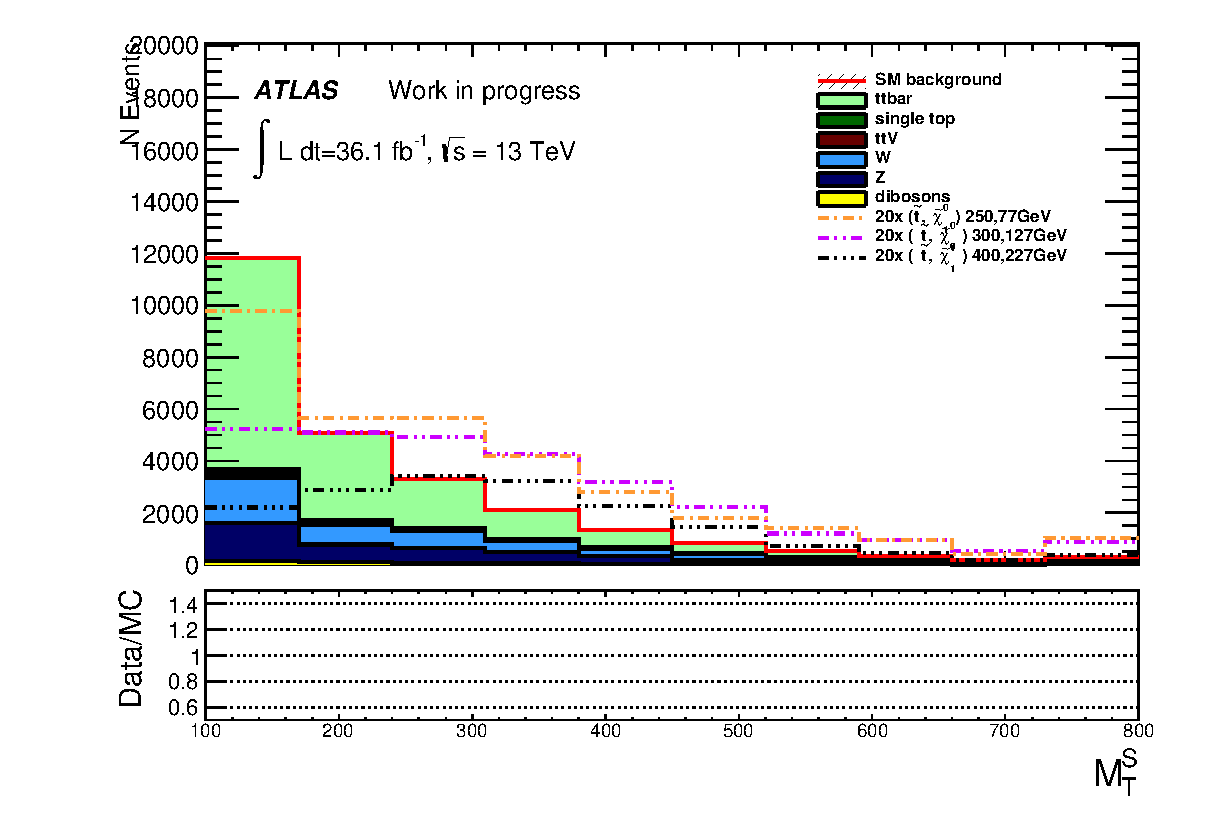
\includegraphics[width=\textwidth]{figures/plotSR/SR_ND1_MS_0SR.eps}%\hspace{0.05\textwidth}
                \caption{ }
    \end{subfigure}
\caption{ (a) $\NjV$ distribution for stop signal and SM background after loose selections for $\met>250 \gev$, zero leptons and at least 4 jets.  (b) $\MS$ distribution for stop signal and background after lose selections for $\met>250 \gev$, zero leptons and at least four jets.  }
\end{center}
\label{fig:gluino_meff} 
\end{figure}

\indent In stop signal, the 6 partons from the two top decays are also boosted by the ISR and tend to go in the same direction as the two neutralinos.  In comparison, the dominant ttbar background tend to have the top and anti-top recoil against one another in a back-to-back fashion.  This leads to only one set of top decay products in the same hemisphere at the $\met$.  Therefore, the signal tends to have higher jet multiplicities and total energy in the hemisphere containing $\met$.  Figure \ref{fig:ISR:ttbarb2b_sig} illustrates this schematically.  \\

\begin{figure}[h!]
  \centering
	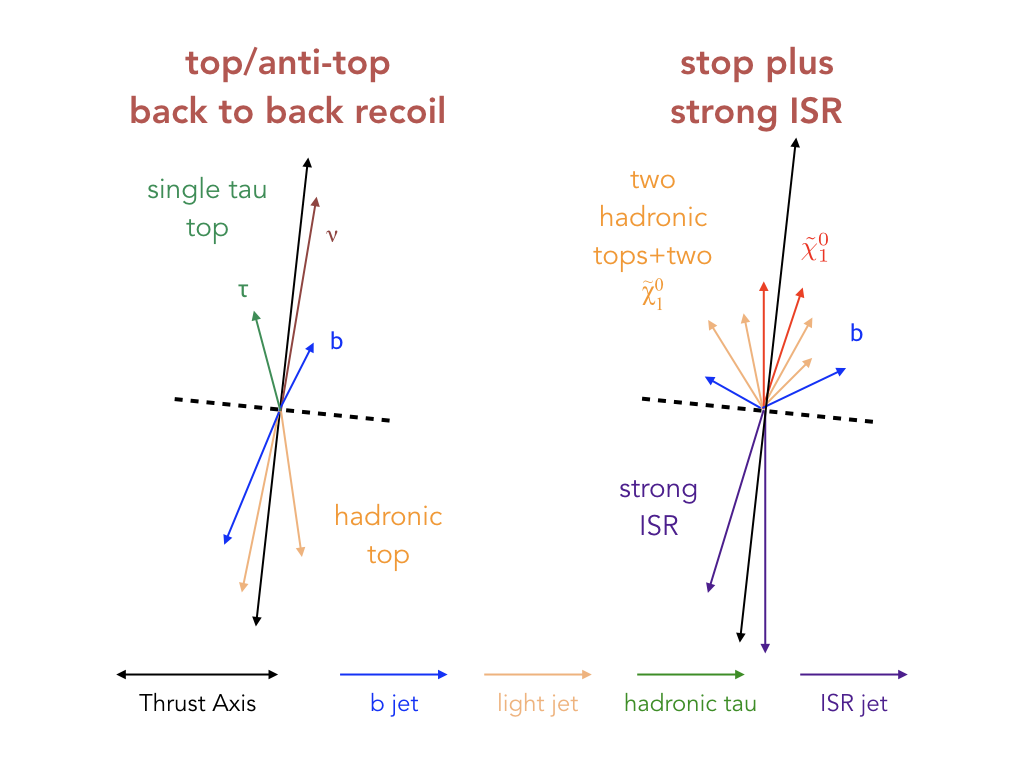
\includegraphics[width=0.85\textwidth]{./figures/strategy/ttbarb2b_stop.png}
	\caption{Schematic depictions of a ttbar top/anti-top back-to-back recoil event and a stop plus strong ISR event.  The thrust axis approximates the direction of back-to-back boost between ISR and stop decay products in signal and the back-to-back boost between the top and anti-top in ttbar background.  This leads to the hemisphere containing $\met$ has greater jet multiplicity $\NjV$ and total transverse mass $\MS$ in signal. }
	\label{fig:ISR:ttbarb2b_sig}
\end{figure}

\indent Chapter \ref{chap:jigsaw} defines the kinematic variables on the sparticle and ISR hemispheres and explains the ISR identification algorithm in greater detail. \\

\indent Selections are made on these sensitive variables forming a signal region (SR) that is optimized to maximize signal sensitivity.  The expected background rates in SR are predicted using a combination of MC and data driven techniques.  One common technique involves making kinematically similar control regions (CR) and validation regions (VR). The CRs are designed to mimic the background kinematics in SR but are orthogonal to SR and are low expected signal rate.  We directly measure the rate of background in the CRs and use simulation to extrapolate background predictions to the SR.  VRs are even closer in kinematic selections to SR and form an independent cross check on the extrapolation between CR and SR. \\

\indent The relationship between CR, SR and VR is graphically depicted in figure \ref{fig:CR_VR_SR_stat1}.  Details on SR selections can be found in chapter \ref{chap:SignalRegion}.  Details on background estimation, CRs and VRs can be found in chapter \ref{chap:backgrounds}. \\

\begin{figure}[h!]
  \centering
	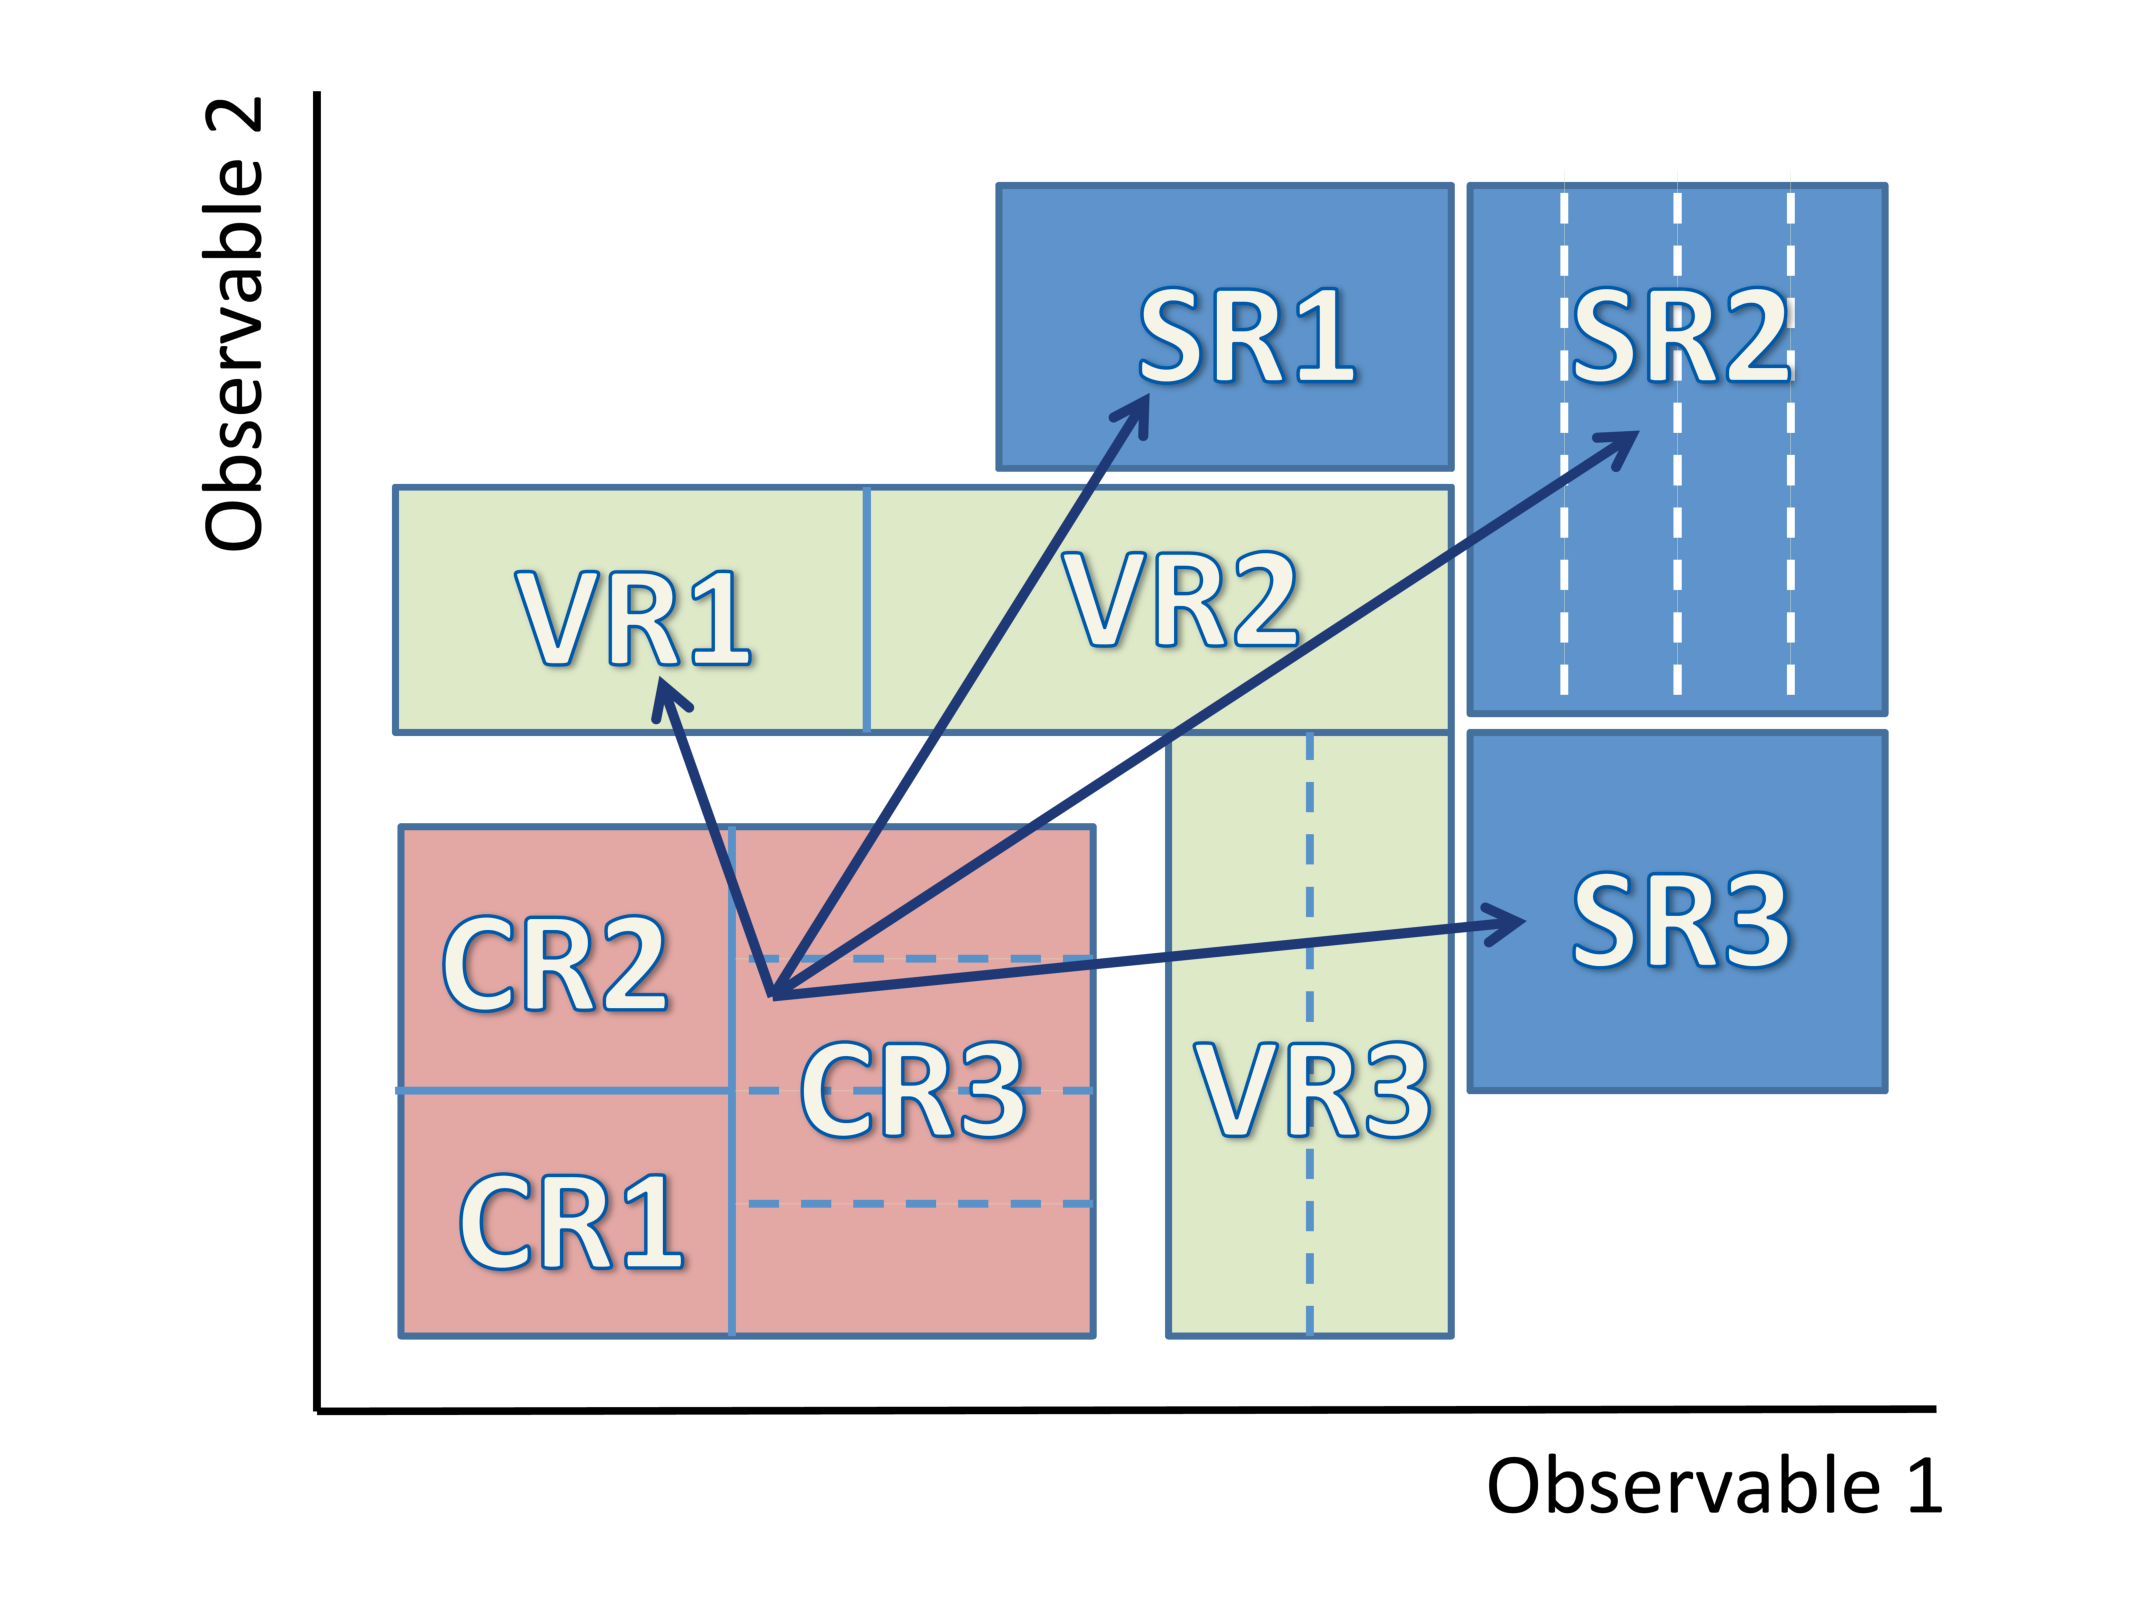
\includegraphics[width=0.65\textwidth]{./figures/statistics/CR_VR_SR.pdf}
\caption{Basic diagram demonstrating the use of control regions (CR) to estimate background rates in the signal region (SR).  We define CR that is dominated by background and have little signal.  We can estimate the amount of background we expect in the SR by measuring the amount of background in the CR and extrapolating to the SR using MC predictions. VRs exist between CRs and SRs and serve as an independent region to validate background predictions.  }
\label{fig:CR_VR_SR_stat1}
\end{figure}

\indent The data in SR is originally blinded to avoid any bias for or against discovery.  We unblind the SR only after we decide the background prediction in SR is well understood based on observations in CRs and VRs. \\

\indent If an excess of data was found in the SR after unblinding then a simultaneous fit to all CR and SR is performed to calculate the statistical significance of any potential excess.   If no excess were found, then a simultaneous fit to all CR and SR is also performed quantify the maximum amount of signal cross-section that can be excluded.  \\
